\documentclass[conference]{IEEEtran}
\usepackage[utf8]{inputenc}
\usepackage[brazil]{babel}
\usepackage{graphicx}
\usepackage{listings}
\bibliographystyle{ieeetr}

\title{Análise evolutiva do Linux através de Design Structure Matrices\\
  \large MATE08 - Tópicos em Engenharia de Software 1 (2012.2)}
\author{Joenio Marques da Costa}
\date{18 de abril de 2013}

\begin{document}
\maketitle

\begin{abstract}
  Este trabalho apresenta um relatório técnico sobre estudo exploratório do
  código-fonte do Linux\cite{WikipediaLinux} a partir de Design Structure
  Matrices (DSM) ao longo de 22 versões do projeto. O objetivo é demonstrar o
  uso de Design Structure Matrices no contexto de software bem como validar a
  ferramenta desenvolvida durante este trabalho. Ao longo de todo o estudo
  faz-se referências ao artigo "Exploring the Strucure os Complex Software
  Designs: An Empirical Study of Open Source and Proprietary
  Code"\cite{ExploringStructure} que deu origem a esta pesquisa e é
  parcialmente reproduzido aqui.

  Palavras-chave: DSM, Analizo, Change Cost, LCOM4.
\end{abstract}

\section{Introdução}

Muitos estudos tem abordado compreensão e visualização de softwares complexos,
dentre estes alguns focam no uso de {\it DSM} a fim de se ter uma visão geral
do relacionamento entre as entidades que compõe o sistema, além de obter meios
para cálculo de métricas como {\it Change Cost}, uma medida que representa o
custo médio de uma mudança no design de um software em termos do potencial
impacto desta mudança em outras partes do sistema.

Este estudo analisa a evolução do Linux e desenvolve ferramentas para geração
de {\it DSM} e para o cálculo da métrica {\it Change Cost} a partir da
ferramenta Analizo\footnote{http://analizo.org}, em seguida faz um comparativo
entre esta e {\it LCOM4}\cite{measuringCouplingAndCohesion}, bem como avalia
os resultados obtidos em relação ao artigo
referência\cite{ExploringStructure}.

\section{Desenvolvimento}

22 versões do Linux foram obtidas através do site
FUNET\footnote{http://www.nic.funet.fi/pub/Linux/kernel} e analisadas através
da ferramenta Analizo\cite{Analizo}, uma ferramenta para análise de código-fonte e
visualização de software. O Analizo no entando não possui suporte a {\it DSM}
ou {\it Change Cost}, portanto foi necessário implementar estes novos recursos
nesta ferramenta\footnote{http://analizo.org/Development/ActionItem34}.

Em resumo as etapas seguidas neste estudo foram as seguintes:

\begin{description}
  \item [1] Implementar suporte a geração de DSM
  \item [2] Desenvolver algoritmo para cálculo de Change Cost
  \item [3] Testar e validar DSM e Change Cost
  \item [4] Analisar o Linux
  \item [5] Traçar um paralelo entre métricas
  \item [6] Avaliar resultados em relação ao artigo referência\cite{ExploringStructure}
\end{description}

\subsection{Implementação e validação}

Uma {\it DSM} é a representação de um grafo de dependência em forma de uma
matriz quadrada, implementar uma ferramenta para este fim se resume a
transformar um grafo em uma matriz e em seguida gerar uma visualização para
esta matriz, isto foi implementado no Analizo a partir do módulo {\it
Graph}\footnote{http://metacpan.org/module/Graph}, uma implementação madura de
estruturas de dados e algoritmos para grafos e do módulo {\it
Graph::Writer::DSM}, um módulo para representação visual de um grafo em forma
de DSM. O resultado desta implementação pode ser visto na Figura~\ref{fig:dsm}.

\begin{figure}[h]
\center
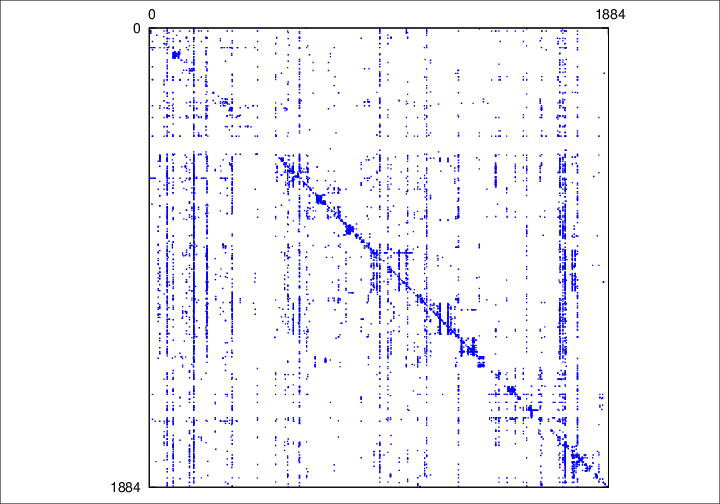
\includegraphics[scale=0.3]{dsm.png}
\caption{Design Structure Matrix do Linux 2.1.105 gerado pelo Analizo}
\label{fig:dsm}
\end{figure}

O {\it Change Cost} representa o impacto que uma mudança localizada em um
certo ponto pode causar em outros pontos do mesmo sistema, ele é calculado a
partir de uma matrix chamada {\it Reachability
Matrix}\cite{ReachabilityMatrices}, foi implementado também através do módulo
{\it Graph} via método {\it transitive\_closure\_matrix}. Por fim calcula-se o
{\it Fan-out} de cada linha da matriz e divide-se pelo total de linhas para
chegar ao resultado final de {\it Change Cost}.

A partir da implementação de {\it DSM} e {\it Change Cost} foram feitas várias
interações para validação da implementação com base em um pequeno contendo
apenas 6 arquivos/módulos.

\subsection{Análise do Linux}

Após validação da implementação iniciou-se a análise de cada versão do Linux
extraindo para cada uma: {\it DSM}, {\it Change Cost},
{\it LCOM4} médio e o número de arquivos, um resumo com todos estes dados
pode ser visto na Tabela~\ref{tab:resumo}. Estes dados foram comparados aos
dados do artigo referência\cite{ExploringStructure} a fim de corrigir
possíveis inconsistências e de se aproximar ao máximo possível dos resultados
encontrados no artigo.

\begin{table}
\caption{Resumo da evolução do Linux}
\centering
\begin{tabular}{| l | c | c | c | c |}
\hline
Versão    & \#Arquivos & Change Cost & LCOM4  \\
\hline
0.01      & 45         & 0.23        & 2.60   \\
0.11      & 52         & 0.33        & 4.66   \\
0.12      & 63         & 0.36        & 4.91   \\
0.95      & 67         & 0.35        & 4.97   \\
0.99.15   & 294        & 0.21        & 4.34   \\
1.0       & 295        & 0.22        & 4.34   \\
1.1.13    & 309        & 0.21        & 3.90   \\
1.1.70    & 358        & 0.26        & 3.59   \\
1.1.95    & 416        & 0.20        & 3.64   \\
1.2.0     & 416        & 0.20        & 3.64   \\
1.2.9     & 416        & 0.20        & 3.75   \\
1.2.13    & 416        & 0.20        & 3.64   \\
1.3.0     & 422        & 0.19        & 3.70   \\
1.3.55    & 585        & 0.21        & 2.13   \\
1.3.100   & 840        & 0.24        & 1.76   \\
2.0       & 874        & 0.23        & 1.71   \\
2.0.34    & 974        & 0.24        & 2.00   \\
2.0.40    & 1082       & 0.25        & 1.65   \\
2.1.0     & 877        & 0.24        & 2.09   \\
2.1.105   & 1885       & 0.18        & 2.64   \\
2.1.132   & 2081       & 0.17        & 2.69   \\
2.2.0     & 1957       & 0.18        & 5.63   \\
\hline
\end{tabular}
\label{tab:resumo}
\end{table}

\subsection{Relação entre métricas}

{\it Change Cost} não indica design bom ou ruim, mas sinaliza em grau de
comparação que um design é mais modular que outro, ou ainda que a
modularização está aumentando ou diminuindo ao longo do tempo. É possível ver na
Figura~\ref{fig:files} por exemplo que o {\it Change Cost} não se altera em
relação ao número de arquivos do projeto.

\begin{figure}[h]
\center
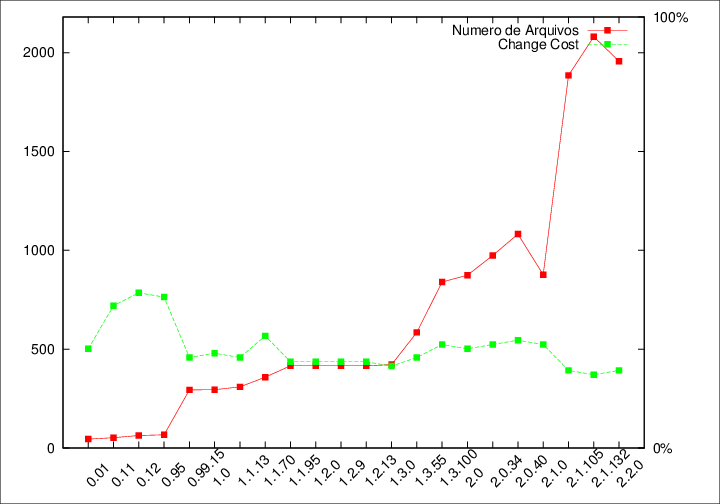
\includegraphics[scale=0.3]{plot-files.png}
\caption{Relação entre Change Cost e Número de Arquivos}
\label{fig:files}
\end{figure}

Assume-se que em designs menos acoplados a medida de {\it Change Cost} também
será menor. A partir desta afirmação é possível relacionar {\it LCOM4 (Lack of
Cohesion in Methods)} com {\it Change Cost}, uma vez que coesão e acoplamento
possuem relação direta. A Figura~\ref{fig:lcom4} mostra o quão próximos se
mantém {\it Change Cost} e {\it LCOM4}, apesar de não ser possível traçar
afirmações sem um estudo aprofundado, intuitivamente estas 2 medidas estão
relacionadas.

\begin{figure}[h]
\center
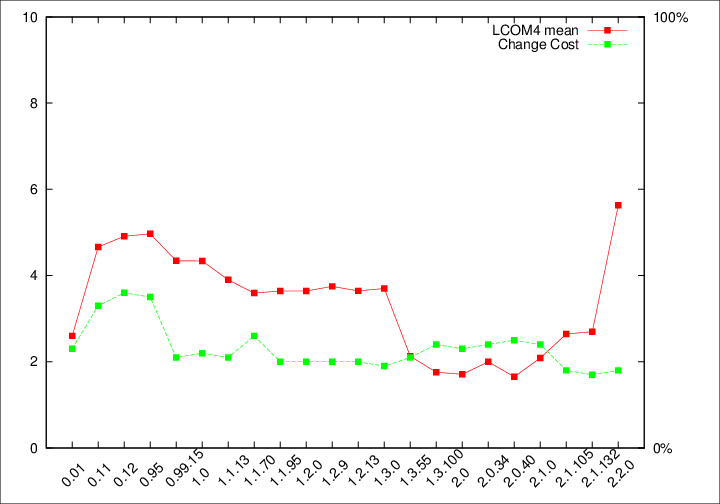
\includegraphics[scale=0.3]{plot-lcom4.png}
\caption{Relação entre Change Cost e LCOM4 médio}
\label{fig:lcom4}
\end{figure}

\section{Conclusões}

Foi ilustrado brevemente como se implementou suporte a {\it DSM} e cálculo de
{\it Change Cost} no {\it Analizo} a partir do estudo evolutivo do Linux
ao longo de 22 versões. Os dados obtidos não são conclusivos uma vez
que o comparativo feito com os valores encontrados no artigo de
referência\cite{ExploringStructure} não coincidem.

Empiricamente é possível levantar dúvidas sobre a validade dos resultados
obtidos no artigo referência\cite{ExploringStructure}, uma vez que o autor não
deixa claro quais ferramentas utilizou para gerar {\it DSM} ou calcular {\it
Change Cost}. O autor calculou por exemplo que o Linux 2.1.105 possui 1678
arquivos e tem {\it Change Cost} = 5.16\%. Ao passo que foi encontrado aqui,
conforme pode ser visto na Tabela~\ref{tab:resumo}, 1885 arquivos e {\it
Change Cost} = 18\% para esta mesma versão.

Este trabalho apresenta uma nova ferramenta para visualização de {\it DSM} e
cálculo de {\it Change Cost} a partir de análise estática baseada no {\it
Analizo} e contribui com uma avaliação parcial dos resultados obtidos no
artigo referência "Exploring the Strucure os Complex Software Designs: An
Empirical Study of Open Source and Proprietary Code"\cite{ExploringStructure}.

\bibliography{bibliografia}
\end{document}
